\documentclass[14pt, a4paper]{extreport}
\usepackage{susu}

% ====================================================================================================
\begin{document}

\author{Алиев~Э.Ф.}
\group{212}
\task{6}
\maketitle

% ====================================================================================================
\chapter{Задание}

\begin{enumerate}

	\item
Написать программу для выполнения аффинных преобразований многоугольника на плоскости. Предварительно определить структуру данных (класс) и разработать соответствующие подпрограммы (методы). Число и координаты вершин многоугольника считать из файла. Интерфейс программы должен содержать следующие элементы управления:
	\begin{itemize}
		\item перемещение фигуры;
		\item поворот фигуры (относительно центра фигуры);
		\item растяжение/сжатие фигуры;
		\item сохранение результата в файл;
		\item выход из программы.
	\end{itemize}

\end{enumerate}

% ====================================================================================================
\chapter{Математическая модель}

структура Point в которой содержится x, y.\\
массив figure типа Point с углами фигуры:

-100 100

0 -100

100 -100

0 100\\
переменная center типа Point с координатами центра: 100, 100.\\
Методы:

void draw(Point, Point*) для отрисовки фигуры.

void scale(Point*, double) для изменения размера фигуры.

void spin(Point*, double) для вращения фигуры.

% ====================================================================================================
\chapter{Текст программы}

\noindent Файл main.cpp
\lstinputlisting{source/main.cpp}
\pagebreak
\hrulefill

\noindent Файл task.h
\lstinputlisting{source/task.h}
\hrulefill

\noindent Файл task.cpp
\lstinputlisting{source/task.cpp}
\hrulefill

\noindent Файл control.h
\lstinputlisting{source/control.h}
\hrulefill

\noindent Файл control.cpp
\lstinputlisting{source/control.cpp}

% ====================================================================================================
\chapter{Результат работы}

\begin{figure}[h!]
	\centering
	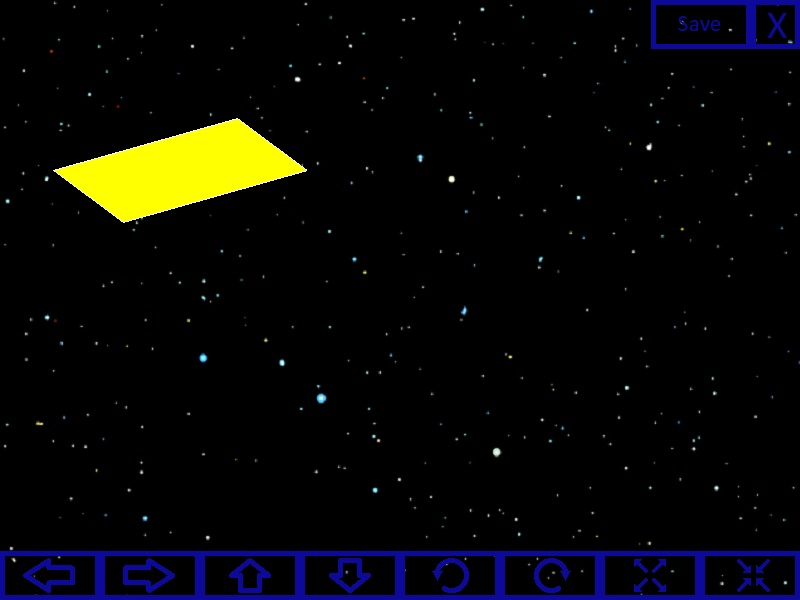
\includegraphics[width = 12cm]{image/output}
  \caption{Результат выполнения программы}
\end{figure}


% ====================================================================================================
\end{document}